\documentclass[12pt,a4paper]{article}
% \usepackage[english]{babel}
% \usepackage[utf8x]{inputenc}

\usepackage{graphicx} % Required for inserting images.
\usepackage[margin=25mm]{geometry}
\parskip 4.2pt  % Sets spacing between paragraphs.
% \renewcommand{\baselinestretch}{1.5}  % Uncomment for 1.5 spacing between lines.
\parindent 8.4pt  % Sets leading space for paragraphs.
\usepackage[font=sf]{caption} % Changes font of captions.
\usepackage{natbib}
\usepackage{amsmath}
\usepackage{amsfonts}
\usepackage{amssymb}
\usepackage{siunitx}
\usepackage{float}
\usepackage{verbatim}
\usepackage{hyperref} % Required for inserting clickable links.
\usepackage{natbib} % Required for APA-style citations.


\title{Do cryptocurrencies extend the mean-variance frontier of an equity investor?}
\author{Sander Naerum, Thomas Pietsch and Ziga Jagodnik}

\begin{document}
\pagenumbering{gobble} %disable page numbering

\maketitle

%adding some space
\vspace{1cm}

\begin{abstract}
\noindent In this project we will investigate if cryptocurrencies extend the mean-variance frontier of an equity investor. 
By using an industry portfolio data set consisting of 12 different industries collected from Kenneth French data library 
combined with the 3 largest cryptocurrencies based on market capitalization, we extract the mean-variance frontier. We show 
that adding cryptocurrencies to the mean-variance frontier has a significant impact.

\end{abstract}

\clearpage
\tableofcontents
\clearpage
\pagenumbering{arabic}
\setcounter{page}{1}

\section{Introduction}\label{sec:intro}
The mean-variance frontier is a mathematical framework for building portfolios that aim to maximize expected returns while 
controlling a set level of risk. This concept extends diversification in investing, highlighting that owning diverse financial 
assets is less risky than focusing on a single asset class. The key idea is that an asset's risk and return should be evaluated 
in the context of its contribution to the overall risk and return of a diversified portfolio. Historical asset price variance 
is used as a proxy for estimating future risk in the mean-variance frontier.

\noindent In the evolving landscape of financial assets, the integration of cryptocurrencies adds a new dimension to portfolio 
construction. Cryptocurrencies, such as Bitcoin and Ethereum, bring unique characteristics and opportunities to the mix. 
Therefore, it is interesting to explore if this new universe of assets can enhance portfolio diversification. 

\section{Methodology}\label{sec:methods}
\subsection{Assumptions under the MPT}
\begin{itemize}
\item Investors prefer higher returns for a given level of risk or aim to minimize risk for a given level of returns.
\item The degree of risk aversion varies among investors.
\item Investors have complete information about expected returns, variances, and covariances for all assets.
\item Investment returns are assumed to follow a normal distribution.
\item Only returns, variances, and covariances are needed to calculate the optimal portfolio.
\item No transaction costs or taxes.
\item All investors can borrow and lend at the same rate. 
\end{itemize}
The mean-variance analysis is used to identify optimal/efficient portfolios.

\subsection{Data}
\textbf{Equity data:} Kenneth French website, 12 industry portfolios. The assets within the industry portfolios are equally 
weighted and the data downloaded has daily frequency. 

\noindent\textbf{Crypto's:} Imported the 3 largest crypto currencies based on market cap, source: Yahoo Finance. Can also be 
extended in the data grabbing. Crypto data is downloaded with daily frequency.  

\noindent \textbf{Caveat:} We only have data from 2017-2023 on the cryptocurrencies. Ideally, to conclude that cryptocurrencies 
actually extends the mean-variance frontier of an equity investor, we would want data on a longer time frame.    

\subsection{Return calculations}
The data downloaded from Kenneth French's website is already calculated as simple returns, and is given in percentage terms. 
To convert them to percentage points we divide them by 100.  

\noindent For the data on the crypto prices downloaded from yahoo finance we use the following formula to obtain the simple 
returns: 
$$r_t = \frac{P_t-P_{t-1}}{P_{t-1}}$$

\subsection{Frontier construction}
\textbf{Consider a three asset portfolio}

Expected return of the portfolio:
$$E(R_p) = w_AE(R_A) + w_BE(R_B) + w_CE(R_c)$$

Portfolio variance: 
\begin{align*} % remove the asterisk to make the equation numbered
\sigma^2_p = & \, w^2_A\sigma^2_A + w^2_B\sigma^2_B + w^2_C\sigma^2_C \\
            & + 2w_A w_B\sigma_A\sigma_B\rho_{AB} \\
            & + 2w_A w_C\sigma_A\sigma_C\rho_{AC} \\
            & + 2w_B w_C\sigma_B\sigma_C\rho_{BC}
\end{align*}


The variance-covariance matrix of assets: 
\[
\text{Covariance Matrix:}
\begin{bmatrix}
    \sigma_{A}^2 & \sigma_{AB} & \sigma_{AC} \\
    \sigma_{AB} & \sigma_{B}^2 & \sigma_{BC} \\
    \sigma_{AC} & \sigma_{BC} & \sigma_{C}^2 \\
\end{bmatrix}
\]

\noindent The mean-variance frontier is found by minimizing the term from (\ref{eq:1}, where $q$ is a given risk tolerance 
factor for an investor, $w$ is a vector of portfolio weights which can also allow for negative values (short). $R$ is a 
expected return vector, and $\sum$ is the variance-covariance matrix. $w^T\sum w$ is the variance of the portfolio return 
and $R^Tw$ is the portfolio's expected return.\cite{wikiref}
\begin{equation}\label{eq:1}
 w^T\sum w - q \cdot R^Tw    
\end{equation}

\noindent The optimization mentioned above identifies a specific point on the efficient frontier. This point corresponds to 
the inverse of the slope of the frontier, that would be $q$, considering a scenario where portfolio return variance is 
plotted horizontally instead of standard deviation. The frontier is parametric on $q$.\cite{wikiref}

\section{Analysis}\label{sec:analysis}
\subsection{Correlations}

From the figure we can conclude that cryptocurrencies have relatively low correlation to the equities and high correlation 
amongst each other. Low correlation would imply that crypto's serves as a good option for diversification for an equity 
investor. However, the small sample size would have to be taken into consideration. 
\begin{figure}[H]
    \centering
    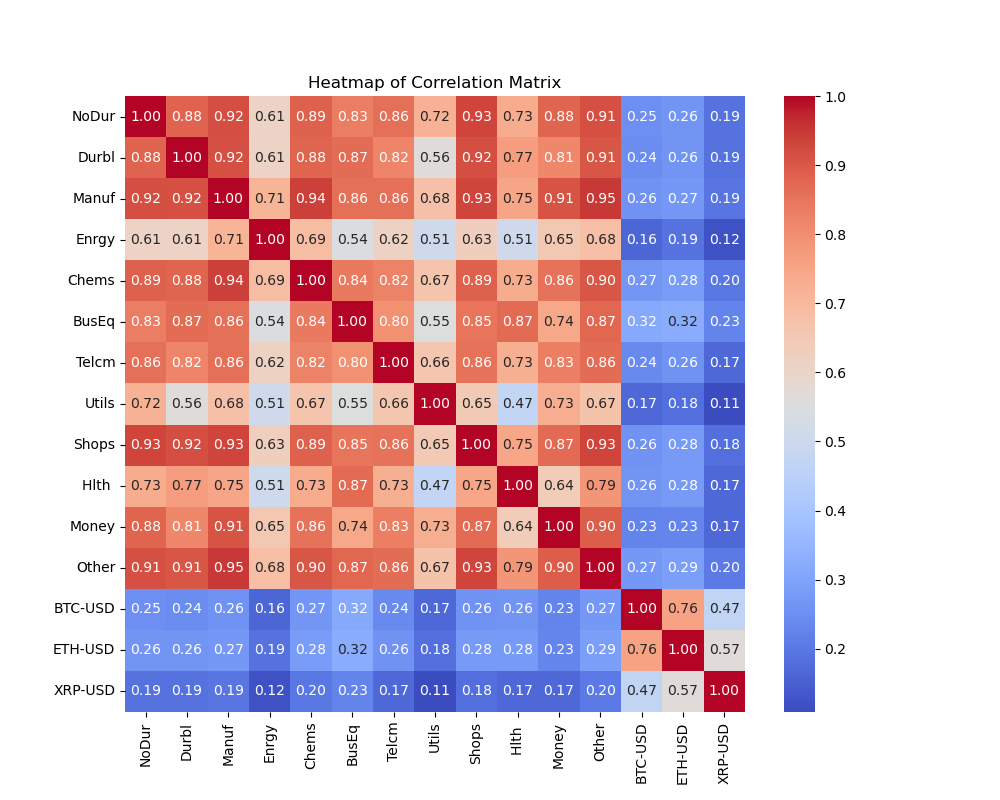
\includegraphics[width=1\linewidth]{Figures/heatmap_correlation.png}
    \caption{Correlations between assets for the full sample}
    \label{fig:correlations}
\end{figure}

\subsection{Sharpe Ratio's}
The Sharpe ratio is defined as: 
$$SR = \frac{E(R_p)-rf}{\sigma_p}$$

\noindent In the Sharpe ratio plot cryptocurrencies are plotted in blue and equities in light blue. From the plot we can tell 
that two of the cryptocurrencies (BTC and ETH) are top performers. The Sharpe ratio measures the excess return you get per 
unit of risk, which also makes it a good proxy as a performance measure. 

\begin{figure}[H]
    \centering
    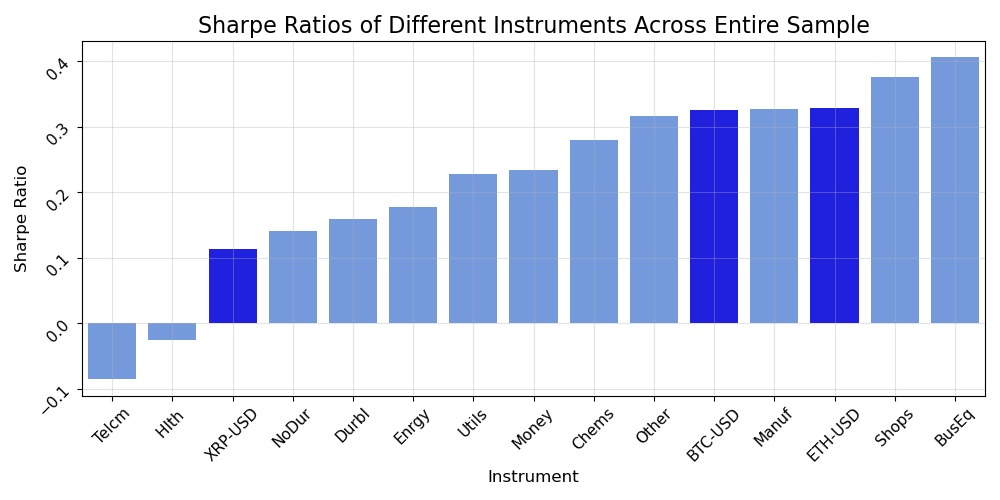
\includegraphics[width=1\linewidth]{Figures/SR_Entire_Sample.png}
    \caption{Sharpe Ratio's for all assets (full sample)}
    \label{fig:Sharpe}
\end{figure}


\section{Results}\label{sec:results}

\subsection{Full Sample}\label{sec:full sample}
\begin{figure}[H]
    \centering
    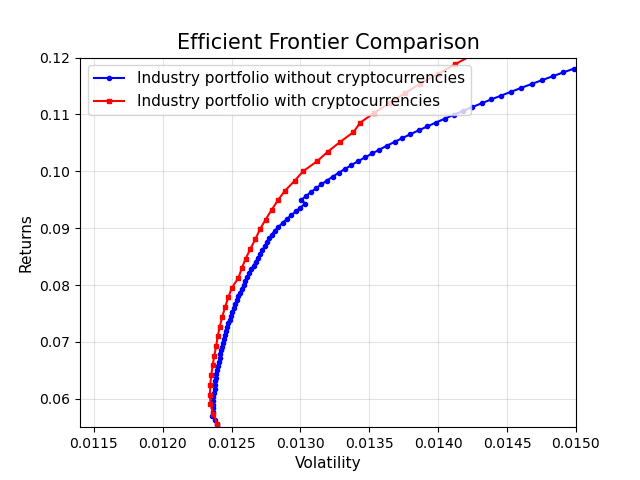
\includegraphics[width=0.9\linewidth]{Figures/Efficient_Frontier_Comparison_Full_Sample.png}
    \caption{Comparing the two mean-variance frontiers for the full sample. From 2017-10-31 to 2023-10-31.}
    \label{fig:full}
\end{figure}

\subsection{Restricted Sample}\label{sec:restricted sample}
\subsubsection{Frontier with equity bull market time frame}
\begin{figure}[H]
    \centering
    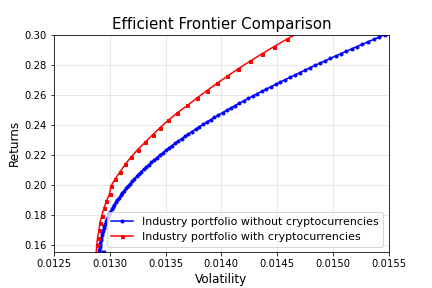
\includegraphics[width=0.7\linewidth]{Figures/Efficient_Frontier_Comparison_Bull_Market.png}
    \caption{Comparing the two mean-variance frontiers for the bull market time frame, from 2017-10-31 to 2021-12-1.}
    \label{fig:bull}
\end{figure}

\subsubsection{Frontier with time frame corresponding to high volatility equity market with large negative drawdowns}
\begin{figure}[H]
    \centering
    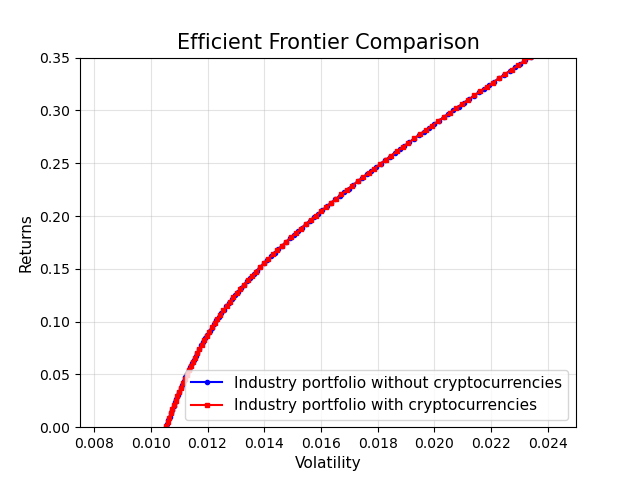
\includegraphics[width=0.7\linewidth]{Figures/Efficient_Frontier_Comparison_Drawdown_Market.png}
    \caption{Comparing the two mean-variance frontiers for the drawdown market, from 2021-12-1 to 2023-10-31.}
    \label{fig:drawdown}
\end{figure}


\section{Conclusion}\label{sec:discussion}
The inclusion of cryptocurrencies in an investment portfolio extends the mean-variance frontier for an equity investor, 
introducing a new dimension to diversification strategies and expanding the spectrum of risk and return possibilities. 
However, the application of modern portfolio theory as a trading strategy is not without criticism. 

\noindent One major critique involves the assumption of normality in MPT, which may not accurately capture the high volatility 
and non-normally distributed returns often exhibited by cryptocurrencies. Additionally, the static nature of expected returns,
 variances, and covariances in the model might not fully account for the dynamic nature of rapidly evolving cryptocurrency 
 markets. The sensitivity of optimal portfolio allocations to input parameters is another concern, as small changes in 
 estimates can lead to significant shifts in portfolio composition.

\noindent Furthermore, the efficiency assumption of market prices in MPT may be challenged in the context of cryptocurrencies, 
where markets may be less mature and subject to information asymmetry.

\clearpage
\addcontentsline{toc}{section}{References}
\bibliographystyle{apalike}
\bibliography{References}

\end{document}
